\documentclass{my_eth_beamer}

\usepackage{my_math_eth}

\numberwithin{equation}{section}

% -----------------------------------------------------------------------------
% this document
\title{Introduction to Survey Sampling}
\newcommand{\TITLE}{Unequal Probability Sampling}
\newcommand{\NR}{5}
\subtitle{Part \NR: \TITLE}
\author[Tobias Schoch]{Tobias Schoch}
\date{2024}

% -----------------------------------------------------------------------------
\begin{document}

\setstretch{1.1}

\section{\TITLE}\label{sec:unequal}
\setcounter{section}{\NR}
\setcounter{Bsp}{17}
\setcounter{Def}{10}
\setcounter{EinSatz}{1}

% -----------------------------------------------------------------------------
\begin{frame}
    \frametitle{Overview}
    \noindent \hspace{0.2em}\textcolor{fhnwblue}{\bfseries \NR~\TITLE}
    \begin{enumerate}[\NR.1]
        \item The Horvitz--Thompson Estimation Principle
        \item Variance Estimation
        \item Probability Proportional to Size (PPS)
        \item Selecting a PPS Sample
    \end{enumerate}
\end{frame}

% -----------------------------------------------------------------------------
\begin{frame}
    \frametitle{\insertsectionnumber~\insertsection}
    Sampling with \alert{unequal} inclusion probabilities (unequal probability
    sampling):

    \vspace{0.25em}

    \begin{itemize}
    \setlength{\itemsep}{8pt}
        \item is of \alert{interest in its own right},
        \item provides the \alert{basis} for formulating a \alert{general theory
            of sampling}.
    \end{itemize}

    \vspace{2em}

    \textbf{\textcolor{fhnwblue}{For orientation}}

    \vspace{0.5em}

    In Chapters 1--4, we followed a \alert{top-down approach}, i.e., we

    \vspace{0.25em}

    \begin{itemize}
    \setlength{\itemsep}{8pt}
        \item specified a \alert{probability distribution} $\PP$ over the set of
            all possible samples $\samplespace$ and
        \item thereby defined the \alert{inclusion probabilities} $\pi_i :=
            \PP(i \in s)$, $i \in U$.
    \end{itemize}
\end{frame}

% -----------------------------------------------------------------------------
\begin{frame}
    In what follows, we take a \alert{bottom-up approach},

    \vspace{0.25em}

    \begin{itemize}
    \setlength{\itemsep}{8pt}
        \item in which the inclusion probabilities $\pi_i$ are assumed to be
            \alert{known} and
        \item serve as the \alert{starting point} for constructing a sampling
            design with these inclusion probabilities.
    \end{itemize}

    \vspace{2em}

    \textbf{\textcolor{fhnwblue}{Motivation}}

    \vspace{0.25em}

    \begin{itemize}
    \setlength{\itemsep}{8pt}
        \item We are interested in estimating the population total
            $\ty = \sum_{i \in U} y_i$.
        \item Recall from Chapter 4 that estimators under \alert{stratified}
            simple random sampling (\STSI) can, under suitable conditions, be
            \alert{more efficient} than under \SRS.
    \end{itemize}
\end{frame}

% -----------------------------------------------------------------------------
\begin{frame}
    \begin{itemize}
    \setlength{\itemsep}{12pt}
        \item Under \STSI, the inclusion probabilities $n_h/N_h$ \alert{differ
            across strata} $h=1,\ldots,H$ (except under proportional
            allocation).
        \item The estimator $\tystrat_{\,}$ under \STSI \alert{compensates} for
            the unequal inclusion probabilities across strata by using the
            \alert{weights} $N_h/n_h$, i.e., the \alert{inverse inclusion
            probabilities}:
            \begin{equation*}
                \tystrat_{\,y} = \sum_{h = 1}^H
                    {\color{magenta}\frac{\bm{N_h}}{\bm{n_h}}} \sum_{i \in s_h}
                    y_i.
            \end{equation*}
        \item We now \alert{generalize} this idea as follows:
            \vspace{0.25em}
            \begin{itemize}
            \setlength{\itemsep}{6pt}
                \item \alert{all} elements $i \in U$ may have \alert{different}
                    inclusion probabilities $\pi_i$,
                \item each observation is \alert{weighted} by the
                    \alert{inverse} $1/\pi_i$.
            \end{itemize}
    \end{itemize}
\end{frame}

\subsection{The Horvitz--Thompson Estimation Principle}

% -----------------------------------------------------------------------------
\begin{frame}
    \frametitle{\insertsectionnumber.\insertsubsectionnumber~\insertsubsection}
    \begin{Def}[\citeauthor{horvitz_thompson_1952},
        \citeyear{horvitz_thompson_1952}]\label{def:sample}

        \vspace{-0.5em}

        Let $p$ be a sampling design without replacement with \alert{possibly
        unequal} inclusion probabilities $\pi_i>0$ ($i\in U$). The
        \alert{Horvitz--Thompson} (HT) estimator of the population total
        $\ty$ is
        \begin{equation}\label{eq:unequal_ht}
            \tysht_{\;y} = \sum_{i \in s} \frac{y_i}{\pi_i}.
        \end{equation}
    \end{Def}
    \begin{itemize}
    \setlength{\itemsep}{10pt}
        \item The estimator should more properly be called the
            \alert{Narain--Horvitz--Thompson} estimator; \citet{narain_1951}
            proposed it ``solely on intuitive grounds'' \citep[][p.
            55]{ajgaonkar_1967}.
        \item \alert{Alternative} representation: \quad $\tysht_{\;y} =
            \displaystyle{\sum_{i \in s}} w_i y_i$ \quad with \quad $w_i =
            \displaystyle{\frac{1}{\pi_i}}$
    \end{itemize}
\end{frame}

% -----------------------------------------------------------------------------
\begin{frame}
    \begin{Exkurs}[Unbiasedness of the HT estimator]
        Let $\indicator_i$ denote the sample inclusion indicator
        $\indicator\{i\in s\}$. It is straightforward to show that the HT
        estimator is \alert{unbiased} for the population total $\ty$ for
        \alert{arbitrary} inclusion probabilities $\pi_i>0$ ($i\in U$):
        \begin{equation*}
            \EE\big(\, \tysht_{\;y}\,\big) = \EE\left(\sum_{i \in U}
            \indicator_i \frac{y_i}{\pi_i}\right) = \sum_{i \in U}
            \EE\big(\indicator_i\big) \frac{y_i}{\pi_i} = \sum_{i \in U} \pi_i
            \frac{y_i}{\pi_i} = \sum_{i \in U} y_i = \ty,
        \end{equation*}
        \noindent where we used $\EE(\indicator_i)=\pi_i$.
    \end{Exkurs}
    \vspace{0.75em}
    \begin{itemize}
    \setlength{\itemsep}{6pt}
        \item The choice of the $\pi_i$ \alert{does}, however, affect the
            variance of the HT estimator.
        \item All estimators discussed so far are \alert{special cases} of the
            HT estimator (e.g., $\tys$ under \SRS or $\tystrat_y$ under
            \STSI).
    \end{itemize}
\end{frame}

% -----------------------------------------------------------------------------
\begin{frame}
    \frametitle{\normalsize Estimating the Population Mean}
    \begin{itemize}
    \setlength{\itemsep}{8pt}
        \item The population mean $\myu$ can be estimated using the HT estimator
            only if $N$ is \alert{known}:
            \begin{equation*}
                \mys^{\;\mHT} = \frac{\tysht_y}{N}.
            \end{equation*}
        \item If $N$ is \alert{unknown}, the \alert{H{\'a}jek estimator} (HJ)
            can be used \citep[][p. 236]{hajek_1971}:
            \begin{align*}
                \mys^{\;\mHJ} &= \frac{\sum_{i \in s} y_i / \pi_i}{\sum_{i \in
                    s} 1 / \pi_i} = \frac{\sum_{i \in s} w_i y_i}{\sum_{i \in
                    s} w_i} && \text{with} \quad w_i = \frac{1}{\pi_i},\\[1em]
                &= \frac{1}{\widehat{N}}\sum_{i \in s} w_i y_i =
                    \frac{\tysht_y}{\widehat{N}} && \text{with} \quad
                    \widehat{N} = \sum_{i \in s} w_i.
            \end{align*}
    \end{itemize}
\end{frame}

% -----------------------------------------------------------------------------
\begin{frame}
    \begin{itemize}
    \setlength{\itemsep}{12pt}
        \item The estimator $\widehat{N}$ can be viewed as the HT estimator of
            $N$ with $y_i\equiv1$, i.e., $\widehat{N}=\sum_{i\in s}1\,w_i$.
        \item The \alert{H{\'a}jek estimator}:
            \vspace{0.25em}
            \begin{itemize}
            \setlength{\itemsep}{8pt}
                \item is a \alert{ratio estimator}

                    \begin{equation*}
                        \mys^{\;\mHJ} = \frac{\tysht_y}{\widehat{N}}
                    \end{equation*}

                    \vspace{0.5em}

                    and is generally \alert{biased} in finite samples,
                    although,
                \item the bias is typically small for sufficiently
                    \alert{large samples}.
                \item is frequently used in practice even when $N$ is
                    \alert{known}.
            \end{itemize}
    \end{itemize}
\end{frame}

\subsection{Variance Estimation}

% -----------------------------------------------------------------------------
\begin{frame}
    \frametitle{\insertsectionnumber.\insertsubsectionnumber~\insertsubsection}
    \begin{Def}[Second-order inclusion probabilities]
        \label{def:inclusionprobabilities_2}
        \vspace{-0.5em}
        Let $p$ be a sampling design without replacement with $\pi_i>0$ for all
        $i\in U$. The probability that elements $i$ and $j$ are both included
        in the sample $s$ is called the \alert{second-order inclusion
        probability} and is defined as
        \begin{equation*}
            \pi_{ij} := \mathbb{P}(i,j \in s) =
                \PP(\indicator_i \indicator_j = 1) \qquad (i,j \in U).
        \end{equation*}
    \end{Def}
    \vspace{0.25em}
    \begin{itemize}
    \setlength{\itemsep}{4pt}
        \item For the \alert{special case} $i=j$, $\pi_{ii}=\pi_i$ for all
            $i\in U$.
        \item For a population of $N$ elements, the matrix of second-order
            inclusion probabilities is of size $(N\times N)$. Because it is
            \alert{symmetric}, it has

            \vspace{-0.7em}

            \begin{equation*}
                \underbrace{N}_{\pi_{ii} = \pi_i} \quad + \quad
                    \underbrace{\frac{N(N - 1)}{2}}_{\pi_{ij}, i < j}
                    \qquad \text{nonredundant entries}.
            \end{equation*}
    \end{itemize}
\end{frame}

% -----------------------------------------------------------------------------
\begin{frame}
    \begin{Def}[Covariance]\label{def:var_cov_indicator}
        \vspace{-0.5em}
        Let $p$ be a sampling design without replacement with $\pi_i>0$ for all
        $i\in U$. The \alert{covariance} $\Delta_{ij}$ between the inclusion
        indicators $\indicator_i=\indicator\{i\in s\}$ and
        $\indicator_j=\indicator\{j\in s\}$, $i,j\in U$, is defined as
        \begin{equation*}
            \Delta_{ij} := \cov(\indicator_i, \indicator_j) = \pi_{ij} -
            \pi_i\pi_j.
        \end{equation*}
    \end{Def}
    \vspace{0.25em}
    \begin{itemize}
    \setlength{\itemsep}{8pt}
        \item Depending on the design, the covariances may be \alert{zero},
            \alert{positive}, or \alert{negative}.
        \item For the variance, $\var(\indicator_i)=\pi_i(1-\pi_i)$ for all
            $i\in U$.
    \end{itemize}
\end{frame}

% -----------------------------------------------------------------------------
\begin{frame}
    \begin{Bsp}[\SRS]
        Under \SRS with sample size $n$ ($0<n<N$), the inclusion probabilities
        are $\pi_i=n/N$ for all $i\in U$ and
        \begin{equation*}
            \pi_{ij} = \frac{n(n - 1)}{N (N - 1)} = \pi_i \, \pi_j \, \frac{N(n
            - 1)}{n(N - 1)} \qquad (\text{for} \;
                i \neq j, \; i, j \in U).
        \end{equation*}

        \vspace{0.25em}

        The \alert{covariance} between the inclusion indicators $\indicator_i$
        and $\indicator_j$ is
        \begin{equation*}
            \Delta_{ij} = \pi_{ij} - \pi_i\pi_j
                = \frac{n(n - 1)}{N (N - 1)} - \left(\frac{n}{N}\right)^2
                = -\frac{f(1 - f)}{N - 1} \qquad (\text{for} \; i \neq j,
                i,j \in U)
        \end{equation*}

        \vspace{0.25em}

        \noindent with $f=n/N$. Since $0<n<N$, we have $0<f<1$. Hence the
        covariance is strictly \alert{negative} for all $i\neq j$.
    \end{Bsp}
\end{frame}

% -----------------------------------------------------------------------------
\begin{frame}
    \begin{itemize}
    \setlength{\itemsep}{15pt}
        \item Let $p$ be a sampling design without replacement with $\pi_i>0$
            for all $i\in U$. The theoretical \alert{variance of the HT
            estimator} is
            \begin{equation*}
                \var\big(\,\tysht\big) = \sum_{i \in U}\sum_{j \in U} \Delta_{ij}
                    \,\frac{y_iy_j}{\pi_i\pi_j}
            \end{equation*}
        \item If $\pi_{ij}>0$ for all $i,j\in U$, then $\var\big(\,\tysht\big)$
            can be estimated by the unbiased \alert{Horvitz--Thompson variance
            estimator} \citep{horvitz_thompson_1952}:
            \begin{equation*}
                \widehat{\var}_{HT}\big(\,\tysht\big) = \sum_{i \in s}
                    \sum_{j \in s} \frac{\Delta_{ij}}{\pi_{ij}}
                    \frac{y_iy_j}{\pi_i\pi_j}.
            \end{equation*}
    \end{itemize}
\end{frame}

% -----------------------------------------------------------------------------
\begin{frame}
    \frametitle{\normalsize Special Case: Fixed Sample Size}
    \begin{itemize}
    \setlength{\itemsep}{12pt}
        \item For a sampling design with \alert{fixed sample size} $n$,
            $\sum_{j\in U}\Delta_{ij}=0$ for all $i\in U$.
        \item Hence, the variance of the HT estimator can also be written as
            \begin{equation*}
                \var\big(\tysht\big) = -\frac{1}{2}
                \sum_{i\in U}\sum_{j\in U}
                \Delta_{ij} \left(
                    \frac{y_i}{\pi_i}-\frac{y_j}{\pi_j}
                \right)^2.
            \end{equation*}
        \item If $\pi_{ij}>0$, this leads to the \alert{Sen--Yates--Grundy}
            \citep[SYG;][]{sen_1953,yates_grundy_1953} variance estimator
            \begin{equation*}
                \widehat{\var}_{SYG}\big(\tysht\big)
                = -\frac{1}{2} \sum_{i\in s}\sum_{j\in s}
                \frac{\Delta_{ij}}{\pi_{ij}}
                \left( \frac{y_i}{\pi_i}-\frac{y_j}{\pi_j}
                \right)^2.
            \end{equation*}
    \end{itemize}
\end{frame}

% -----------------------------------------------------------------------------
\begin{frame}
    \begin{itemize}
    \setlength{\itemsep}{6pt}
        \item If $\Delta_{ij}\leq0$ for all $i\neq j$, $i,j\in U$, the SYG
            estimator is \alert{nonnegative}.
        \item The SYG estimator is \alert{numerically more stable} than
            $\widehat{\var}_{HT}$, particularly when the coefficient of
            variation of the $y_i/\pi_i$ is small.
        % \item If $\pi_{ij}=0$ for some $i\neq j$, the SYG estimator cannot be
        %     computed as stated. Omitting such pairs generally leads to
        %     \alert{downward bias}.
    \end{itemize}
    \vspace{1em}
    \begin{Exkurs}[Important identities]
        \vspace{0.25em}
        For sampling designs $p$ with \alert{fixed sample size} $n$,
        \begin{equation*}
        \sum_{i\in U}\pi_i=n
        \qquad\text{and}\qquad
        \sum_{j\in U}\pi_{ij}=n\pi_i
        \quad (i\in U).
        \end{equation*}
        Hence,
        \begin{equation*}
        \sum_{j\in U}\Delta_{ij}
        =
        \sum_{j\in U}(\pi_{ij}-\pi_i\pi_j)
        =0
        \qquad (i\in U).
        \end{equation*}
        \vspace{0.25em}
    \end{Exkurs}
\end{frame}

% -----------------------------------------------------------------------------
\begin{frame}
    \begin{Exkurs_forts}[cont.]
        \vspace{0.25em}
        \begin{itemize}
        \setlength{\itemsep}{12pt}
            \item In other words,
                \begin{equation*}
                    \text{fixed $n$} \quad \Longrightarrow \quad
                    \sum_{j} \pi_{ij} = n \pi_i \quad \Longrightarrow \quad
                    \sum_{j} \Delta_{ij} = 0 \quad \Longrightarrow \quad
                    \text{SYG representation}
                \end{equation*}
            \item The above identities are useful for checking inclusion
                probabilities and lead to the Sen--Yates--Grundy representation
                of the HT variance.
        \end{itemize}
    \end{Exkurs_forts}
\end{frame}

% -----------------------------------------------------------------------------
\begin{frame}
    \frametitle{\normalsize Approximation of Second-Order Inclusion
        Probabilities}
    \begin{itemize}
    \setlength{\itemsep}{8pt}
        \item \citet{brewer_2000} proposed the following \alert{approximation}
            of second-order inclusion probabilities for \emph{high-entropy}
            designs:
            \begin{equation}\label{eq:unequal_brewer_pij}
                \pi_{ij} \approx \pi_i \, \pi_j \, \left(\frac{c_i +
                    c_j}{2}\right) \qquad (i,j \in U, \; i \neq j),
            \end{equation}
            \noindent where the choice of the constants $c_i$, $i\in U$, is
            discussed below.
        \item Systematic sampling, for example, has low entropy.
        \item Based on the approximation in
            (\ref{eq:unequal_brewer_pij}), \citet{brewer_2000} gave the
            following approximation to the theoretical \alert{variance of the
            HT estimator}:

            \vspace{-0.5em}

            \begin{equation*}
                \var_{\mathrm{A}}\big(\,\tysht\big) = \sum_{i \in U} \pi_i
                    \big(1 - c_i \pi_i\big)
                    \left(\frac{y_i}{\pi_i} - \frac{\ty}{n} \right)^2.
            \end{equation*}
    \end{itemize}
\end{frame}

% -----------------------------------------------------------------------------
\begin{frame}
    \begin{itemize}
    \setlength{\itemsep}{12pt}
        \item He also recommended the following \alert{variance estimator}:
            \begin{equation*}
                \widehat{\var}_{\mathrm{A}}\big(\,\tysht\big) = \sum_{i \in s}
                    \left(\frac{1}{c_i} - \pi_i\right)
                    \left(\frac{y_i}{\pi_i} - \frac{\tysht_y}{n} \right)^2.
            \end{equation*}
            \begin{itemize}
            \setlength{\itemsep}{6pt}
                \item The variance estimator is asymptotically unbiased for
                    $\var_{\mathrm{A}}\big(\,\tysht\big)$.
                \item $\widehat{\var}_{\mathrm{A}}\big(\,\tysht\big)$ is easy
                    to compute.
            \end{itemize}
        \item \citet{brewer_2000} proposed \alert{three variants} for choosing
            the \alert{constants} $c_i$. We use Variant 1:
                \begin{equation*}
                    c_i  = \frac{n - 1}{n - \pi_i} \qquad (i \in U).
                \end{equation*}
    \end{itemize}
\end{frame}

\subsection{Probability Proportional to Size (PPS)}

% -----------------------------------------------------------------------------
\begin{frame}
    \frametitle{\insertsectionnumber.\insertsubsectionnumber~\insertsubsection}
    \begin{Bsp}[Oracle, Population U14]\label{ex:unequal_oracle}
        \begin{center}
        {\scriptsize
        \begin{tabularx}{\textwidth}{Xrrrrrrrrrrrrrr}
            \addlinespace
            \footnotesize{$i$:} & 1 & 2 & 3 & 4 & 5 & 6 & 7 & 8 & 9 & 10 & 11 &
            12 & 13 & 14\\
            \addlinespace
            \midrule
            \addlinespace
            \footnotesize{$y_i$:} & $175$ & $143$ & $116$ & $85$ & $150$ & $92$
            & $108$ & $67$ & $121$ & $99$ & $118$ & $259$ & $75$ & $142$\\
            \addlinespace\addlinespace
            \footnotesize{$\pi_i$:} & $\displaystyle{\frac{2}{5}}$ &
            $\displaystyle{\frac{286}{875}}$ & $\displaystyle{\frac{232}{875}}$
            & $\displaystyle{\frac{34}{175}}$ & $\displaystyle{\frac{12}{35}}$
            & $\displaystyle{\frac{184}{875}}$ &
            $\displaystyle{\frac{216}{875}}$ & $\displaystyle{\frac{134}{875}}$
            & $\displaystyle{\frac{242}{875}}$ &
            $\displaystyle{\frac{198}{875}}$ & $\displaystyle{\frac{236}{875}}$
            & $\displaystyle{\frac{74}{125}}$ & $\displaystyle{\frac{6}{35}}$ &
            $\displaystyle{\frac{284}{875}}$ \\
        \end{tabularx}
        }
        \end{center}
        \vspace{0.5em}
        A probability sample of size $n=4$ is selected without replacement
        from U$14$. The \alert{realized} sample $s$ is
        \begin{align*}
            y_1 &= 175,& y_2 &= 143,& y_8 &= 67,& y_{14} &= 142\\
            \pi_1 &= \frac{2}{5},& \pi_{2} &= \frac{286}{875},&
            \pi_{8} &= \frac{134}{875},& \pi_{14} &= \frac{284}{875}.
        \end{align*}
    \end{Bsp}
\end{frame}

% -----------------------------------------------------------------------------
\begin{frame}
    \begin{Bsp_forts}[Cont.]
        \vspace{0.25em}
        \begin{itemize}
        \setlength{\itemsep}{8pt}
            \item For the realized sample, the HT estimator gives
                \begin{equation*}
                    \tysht_{\;y} = \sum_{i \in s} \frac{y_i}{\pi_i} = 1'750.
                \end{equation*}
            \item The estimate $\tysht_{\;y}$ equals the true population total
                $\ty$.
            \item The variance of the estimator is zero,
                $\var(\,\tysht_{\;y})=0$; hence there is \alert{no sampling
                uncertainty}.
            \item In this application, the HT estimator has zero variance
                because the inclusion probabilities $\pi_i$ were constructed
                by an \alert{oracle}, assuming that all $y_i$ ($i\in U$) were
                already \alert{known before sampling}.
            \item Clearly, this makes the idea of estimation \alert{absurd}.
        \end{itemize}
    \end{Bsp_forts}
\end{frame}

% -----------------------------------------------------------------------------
\begin{frame}
    \begin{Bsp_forts}[Cont.]
        \vspace{0.25em}
        \begin{itemize}
        \setlength{\itemsep}{2pt}
            \item We can nevertheless learn something from this \alert{absurd}
                situation.
            \item The first-order inclusion probabilities $\pi_i$ were chosen
                \alert{proportional} to the $y_i$:

                \vspace{-0.75em}

                \begin{equation*}
                    \pi_i = \frac{n y_i}{\sum_{i \in U} y_i} = \frac{n
                    y_i}{\ty} \qquad (\text{for all} \; i \in U),
                \end{equation*}
                \noindent so that the HT estimator becomes
                \begin{equation*}
                    \tysht_{\;y} = \sum_{i \in s} \frac{y_i}{\pi_i} = \sum_{i
                    \in s} \frac{y_i}{n y_i} \ty = \ty.
                \end{equation*}
        \end{itemize}
    \end{Bsp_forts}
        \begin{itemize}
        \setlength{\itemsep}{6pt}
            \item Let $x_i$ be an \alert{auxiliary variable} known for
                \alert{all} $i\in U$.
            \item For example, $x_i=$ number of employees in business $i$
                (auxiliary variable known from a register), and $y_i=$ revenue
                (variable of interest, unknown).
        \end{itemize}
\end{frame}

% -----------------------------------------------------------------------------
\begin{frame}
    \begin{itemize}
    \setlength{\itemsep}{11pt}
        \item Assume that $y_i$ and $x_i$ are strongly \alert{positively
            correlated}.
        \item We consider a fixed-size sampling design. If $y_i\propto x_i$,
            then $\var\big(\tysht_{\;y}\big)=0$; see the artificial situation
            in Example \ref{ex:unequal_oracle}.
        \item The first-order \alert{inclusion probabilities} are chosen
            proportional to size (PPS), i.e.,
            \begin{equation*}
                \pi_i = \frac{n x_i}{\sum_{i\in U}x_i}
                \qquad (i\in U),
            \end{equation*}
            provided that $0<\pi_i\leq1$ for all $i\in U$.
        \item Variable $x_i$ is called the \alert{measure of size} (e.g.,
            number of employees).
        \item If proportionality is not exact, PPS sampling can still yield
            \alert{efficiency gains} over \SRS when $x_i$ is strongly related
            to $y_i$.
    \end{itemize}
\end{frame}

% -----------------------------------------------------------------------------
\begin{frame}
    \frametitle{\normalsize Example (Data from Example
        \ref{ex:unequal_oracle})}
    \begin{center}
        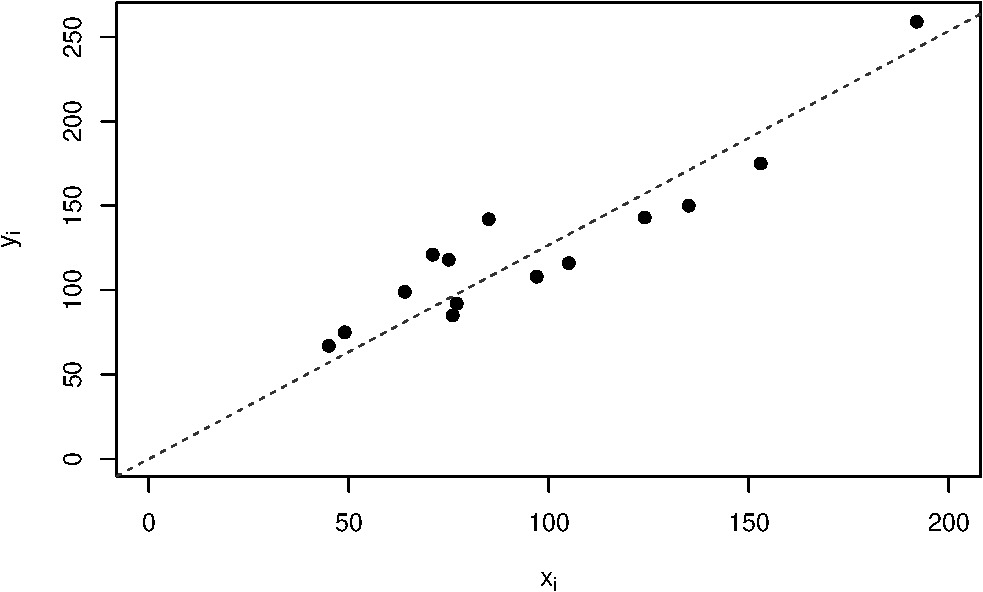
\includegraphics[width=0.8\textwidth]{figures/unequal_rao_1963}
    \end{center}
\end{frame}

\subsection{Selecting a PPS Sample}

% -----------------------------------------------------------------------------
\begin{frame}
    \frametitle{\insertsectionnumber.\insertsubsectionnumber~\insertsubsection}
    \begin{itemize}
    \setlength{\itemsep}{8pt}
    \item \citet{hanif_brewer_1980} classified \alert{47} PPS sampling
        procedures without replacement; for more recent literature, see
        \citet{tille_2006}.
        \item Following their classification, we impose the following
            \alert{requirements} on PPS designs (for all $i,j\in U$):
            \vspace{0.25em}
            \begin{itemize}
            \setlength{\itemsep}{6pt}
                \item \alert{fixed} sample size $n$;
                \item the $\pi_i$ are strictly \alert{proportional} to $x_i$;
                \item \alert{unbiased} variance estimation: $\pi_{ij}>0$
                    for all $i\neq j$;
                \item the SYG variance estimator is \alert{nonnegative}:
                    $\Delta_{ij} \leq 0$ for all $i\neq j$.
            \end{itemize}
    \item The sampling procedure of \citet{brewer_1963,brewer_1975} satisfies
        these requirements (first procedure).
    \end{itemize}
\end{frame}

% -----------------------------------------------------------------------------
\begin{frame}
    \frametitle{\normalsize{Sampling Procedure of \citet{brewer_1963}; Sample
    Size $n=2$}}

    \alert{Assumption:} $x_i<\tx/2$ for all $i\in U$. Then
        \begin{equation*}
            \pi_i=\frac{2x_i}{\tx}<1 \qquad (i\in U).
        \end{equation*}

    \vspace{-0.5em}

    \begin{enumerate}[1)]
    \setlength{\itemsep}{6pt}
        \item Select the \alert{first element} with probability
            \begin{equation*}
                p_i = \frac{c_i}{\sum_{i \in U}c_i}, \qquad
                c_i = \frac{x_i (\tx - x_i)}
                {\tx (\tx - 2 x_i)}
                \qquad (i \in U).
            \end{equation*}
            Denote the selected element by $k$; it is not replaced.
        \item Select the \alert{second element} with conditional probability
            \begin{equation*}
                p_{j \mid k} = \frac{x_j}{\tx - x_k},
                \qquad j\in U\setminus\{k\}.
            \end{equation*}
    \end{enumerate}
\end{frame}

% -----------------------------------------------------------------------------
\begin{frame}
    \begin{itemize}
    \setlength{\itemsep}{8pt}
        \item \citet{brewer_1963} derived a formula for the
            \alert{second-order inclusion probabilities}.
        \item In the \alert{general case}, i.e., when $n>2$,
            \vspace{0.25em}
            \begin{itemize}
            \setlength{\itemsep}{6pt}
                \item the prescribed PPS inclusion probabilities
                    \begin{equation*}
                        \pi_i = \frac{n x_i}{t_x}
                    \end{equation*}
                    require $x_i\le t_x/n$ for all $i\in U$;
                \item units with $\pi_i=1$ are \alert{certainty units} and are
                    included in the sample with probability one;
                \item after removing certainty units, the inclusion
                    probabilities for the remaining units must be recalculated;
                \item sample selection is substantially more \alert{involved};
                    see \citet{brewer_1975}.
            \end{itemize}
    \end{itemize}
\end{frame}



% -----------------------------------------------------------------------------
\setcounter{section}{\the\numexpr\value{section}-1\relax}
\begin{frame}[allowframebreaks]
    \frametitle{References}
    {\footnotesize
        \setstretch{1.1}
        \bibliographystyle{fhnw_en}
        \bibliography{master}
    }
\end{frame}

% -----------------------------------------------------------------------------
\lastpage

\end{document}
